\chapter{Cardioline Specific ecosystem}
\label{chapter:cardioline_specific_ecosystem}
Cardioline is present on the market from the early 60s, they started developing and producing innovative machines to record the heart activity. Nowadays their technology improved, making their products producing documents in a digital format.
Thus the company started to sell an ecosystem composed by its products. Currently they provide heart rate monitor machines which produce digital documents, software tools to forward them to management system and client application or web based application to carry out the exam lifecycle.

\section{Software and Frameworks involved}
Because Cardioline SCP-ECG libraries are microsoft technologies based, their software are based on .NET platform.
The current Cardioline management software is a 3-tier MVC web application written in C\# and deployed on windows server running machines.

\section{Project target And Requirements}
The scope is to provide future customers with additional features with respect to the current offered Ecosystem, avoiding the burden to keep up and running their own machines and infrastructure while Respecting the European jurisprudence in privacy subject and integrating their system with the national e-healthcare system. The company would like to supply their customer physicians and technicians with an electrocardiograph in order to make them perform cardio tests on their patients.\\
Later the documents should be uploaded to a customer dedicated cloud repository and an expert enabled to report it. Finally the user who submitted the exam can access the application and view the physician conclusions.
To carry out the target, these were the main challenges:
\begin{itemize}
    \item High network and computing load
    \item New security policies for data
    \item Adoption of the international HL7 standard
    \item Continuity with legacy software
\end{itemize}
The resulting prototype had to be sufficiently flexible and configurable to be adapted over several environments.

\subsection{Functional and Non functional requirements} As reported above, Cardioline together with academic and research partners came up with additional features which the current version of their system does not support.\\The following are the functional requirements.
\paragraph{Anamnesis}The future management system should let the single tenant decide wether or not to allow cardiologist submit their report even if the patient doctor didn't upload the exam with an anamnesis description. This feature is in particular important for pharmacies, because their technicians are not qualified to insert patient anamnesis. In this way every Cardioline customer (which correspond to hospital, clinic, etc..) can exert its own policy about anamnesis and reviews.
\paragraph{Notifications}Currently Cardioline web application software does not provide a notification features, mainly because it is hosted on LANs.\\Because the architectural change enabled ubiquitous examination and analysis, it also imposes the development of a reliable notification system. Once a new electrocardiogram is submitted, if the system is in this way configured, a notification is sent to users which have anamnesi providing rights on it. If the option is not activated by the tenant user with exam review privileges are notified.\\In the case an anamnesis is submitted, the associated physician are notified for a new available ECG.\\Finally when an ECG review is submitted by physician, the user who is taking care of the associated patient receives a notification of the process completion.

Non-functional requirements are mainly necessary because of the cloud environment introduction and does not affect the system behaviour already implemented.

\paragraph{Legacy software constraints}
Reuse previously implemented software modules and avoid prototype development from scratch.
\paragraph{Scalability}
Dynamically allocate resources to satisfy system traffic and computational load even in case it decreses or increase. The aim to keep stable the level of performance and efficiency adapting to the current workload.\\
\paragraph{Multiple tenants}
Because of application logic and security issues each tenant related data have to be stored in several databases. In this way each tenant can only access its own data.
\paragraph{Availability}
Build a web application which probability of downtime and single point of failures are minimized. Also hardware and network failures have to be prevented.

\paragraph{Legal constraints}
Store data on remote environment rather than a local one implies a different legislation to be applied. Even if EcgWebApp was already compliant to the European laws it had to be reviewed, in particular the database had to be encrypted and modified in order to separate user identifying data and their associated exams.



\section{Proposed solutions}
\label{section:proposed_solutions}
Several solutions were elaborated and proposed to the company, each of them respects the above requirements.\\
Amazon was choosen as service provider because it not only offers storage servers located in Europe, but they are also CISPE certificated: they ensure data be processed and saved into European Union lying servers.\\
Their cloud servers locations are spread around 18 regions over the world, other four have been planned for the next future. Hence it is easier to store physically data for an Amazon customer and make the service compliant to the local legislation. In case of an expansion of Cardioline system, thanks to the cloud region structure the process will be simplified. In figure \ref{fig:amazon_cloud_region} it is possible to observe where Amazon cloud regions are located and where did they plan to host the future ones.
\begin{figure}[h]
    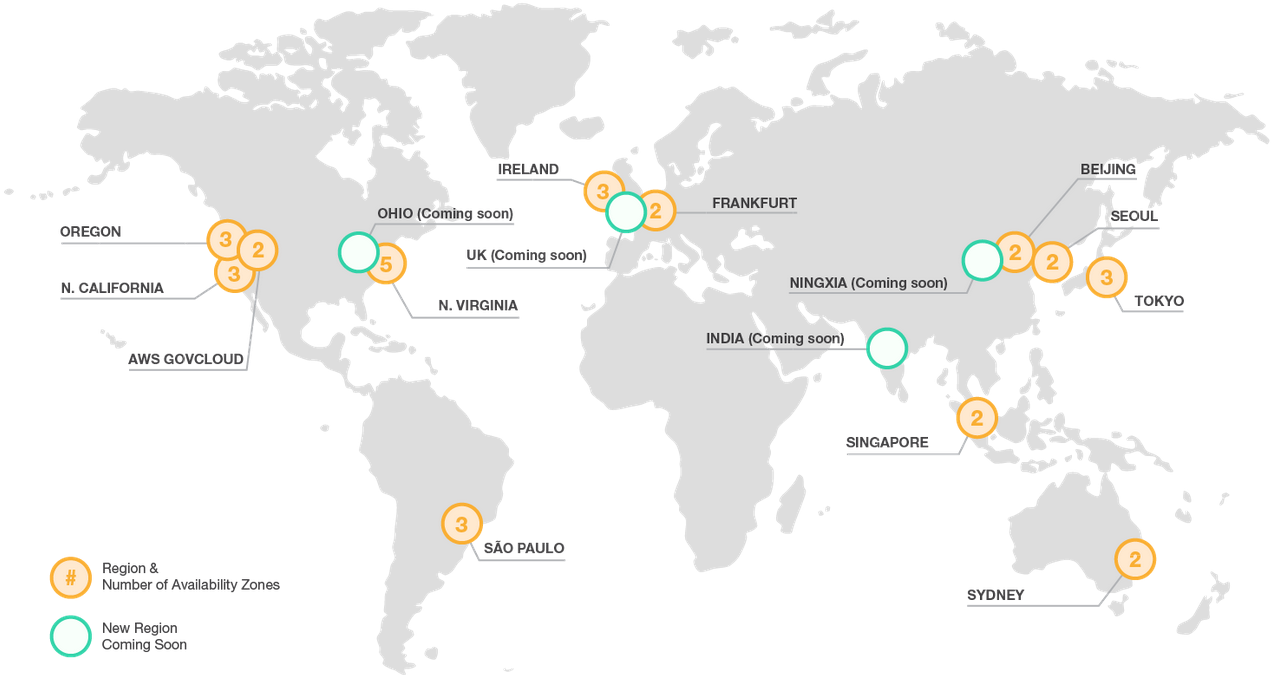
\includegraphics[width=\textwidth,keepaspectratio]{img/amazon_cloud_regions}
    \caption{Geographical location of the different Amazon Cloud Regions}
    \label{fig:amazon_cloud_region}
\end{figure}

Farther the provider was interesting for a particular service they offer named Elastic Beanstalk \label(definition:beanstalk): it allows to manage web and application service. Handles dynamically the computing and network resources allocated to each application, indeed it provides the admin with a real-time monitoring of the applications state. Everything is carried on by Beanstalk leaving the possibility to go deeply and handle directly AWS resources as if the system were PaaS instead.\\
The entire cost is computed by summing up just the usage of AWS resources, meaning that Beanstalk does not provide additional costs to manage automatically the underlying IaaS.
In this phase was also took into account a third party service called \textit{chino.io} so to outsource the storage of sensible data. Chino was granted to be laws compliant in term of privacy, security and easy to integrate by adding an external REST adapter toward their service.
Here are the proposals brought to the company:
\begin{itemize}
    \item Public cloud - PaaS - Amazon RDS - Amazon S3
    \item Public cloud - Elastic Beanstalk - Amazon RDS - Amazon S3
    \item Public cloud - PaaS - third party storage service - Amazon EC2
\end{itemize}
Based on the first analysis phase and according to the company, it has been decided to start working with Amazon Elastic Beanstalk (IaaS) deployed on a public cloud and Amazon RDS / Amazon S3 as storage cloud services.